% !TEX root = ../main.tex
\section{The Survey}\label{sec:survey}
  
  The problem with analyzing passwords is that you need to actually have passwords to analyze. The majority of published research on passwords are often using passwords for leakage or getting passwords distributed from legal sources. Looking at the Android lock pattern there exists no distributed sources, and all lock patterns are only stored locally on each device. 

  People working with security are striving to teach people about security, and one of the rules everyone probably know about is that you should never share a password because it is a secret you should keep to yourself. In this research I have to be a hypocrite and do the opposite; I need to ask people to share their secrets in the name of science. 

  This section will include a detailed description of how the custom made survey was created and how it works. The survey is created for collecting Android Pattern Locks and other background data from the users on mobile devices. 

  \subsection{Requirements}

    When coping with the difficulties with collecting data it is important to define requirements for the survey application. This section will not go through a predefines list of requirements, rather elaborate and discuss the requirements in general to be able to explain its importance.

    \subsubsection*{Language and communication}
      - ordbruk: korte setninger for at folk skal gidde å lese.
      - ordbruk: spørsmålene må være formulert på en måte slik at alle forstår (unngå tekniske uttrykk)
      - Unngå lange setninger
      - Unngå at personer føler seg utrygge eller dumme fordi de ikke kan svare.  (treningsmodus og valgalernativer som fører personen ut av en ukomfertabel sone, men samtidig gi data som kan brukes. )
      - Naturlig valg å bruke engelsk, men ikke alle kan engelsk --> kommuniserer spørsmålet med ikoner. 
      - Cross-cultural requirements
      - Kan ikke anta at alle vet hva låsemønster og android er

    \subsubsection*{Trustworthiness}
      - Tilgjengeliggjøre meg selv via nettside og kontaktinformasjon. Det er virktig å vise at det kommer fra en seriøs kilde og det er viktig å vise hvem som spør om hjelp. Må fremstå som pålitelig og lite skummel. 
      - Fargebruk og bilder må virke lite skumle. 
      - Lage et eksempel på et bilde med mørke farger og et med lyse farger for å hvise at det har mye å si på hvordan man kommuniserer ut til bruker. 
      - Vise til hvem som mottar og behandler data

    \subsubsection*{Technical device and environment of use}
      - Andorid brukes bare på små enheter
      - Vil ikke samle inn data som ikke er generert fra det miljøet det vanligvis brukes. Mulig man kan få flere svar med å samle inn data på desktop, men dataen mister credability. Basert på analysen av hvilke egenskaper som skal inkluderes kan ikke de anlyseres om spørreundersøkelsen ikke blir tatt på en mobil enhet. 
      - Setter høye krav til kontroll
      - Setter høye krav til brukergrensesnitt
      - Utelukker muligens noen brukere som ikke eier en smarttelefon, men kan anta disse som ikke relevante for sample siden de ikke eier teknisk utstyr som er nødvendig. 
      - Mister kontroll på hvem som svarer, men styrker også anonymitet fordi jeg ikke har mulighet til å sjekke hvem som svarer.

    \subsubsection*{Complexity and length}
      - Hvis undersøkelsen blir for lang er det fare for at mange vil avbryte undersøkelsen før den er ferdig
      - Selv om man kommer med prevantive tiltak mot lang undersøkelse er det viktig å prioritere spørsmålene etter prioritert rekkefølge (viktighet av spørsmål).
      - Det er veldig viktig at ingen føler seg dumme når de gjennomgår spørreundersøkelsen. Det kan komme tilfeller der personer som ikke har brukt løsemønster vil svare. Det er defor lagt til treningsmodus for at alle skal føle mestring og unngå frustrasjon.
      - Som nevnt på språk og kommunikasjon er det viktig at spørsmålene er lette og korte der man også unngår kompliserte ord og tunge faguttrykk.
      - Lengde og data nødvendig for å kunne analysere data

    \subsubsection*{Visual appearance and psychology}
      - Å li bedt om å lage mønster/password kan for mange virke som en avskrekkende ting. Det er derfor virkig å utnytte psykologien! Bruk farger som virker imøtekommende og som ikke forbindes med noe farlig. 
      - Ikoner kan også hjelpe å gi undersøkelsen et "barnslig" preg som også gjør at det virker mindre skummelt
      - Viktig å vise hvem jeg er og at jeg kan stoles på. Dette er nevnt tidligere, men vis tydelig bilde slik at personer får tiltro. Hjemmesiden min er laget rosa fordi 1) det faktisk representerer meg 2) det virker ikke skummelt.
      - Gjøre meg tilgjengelig.
      - Finnes det noe fargeteori som kan refereres til?
      - Finnes det noe forskning på hva man må gjøre når man lager spørreundersøkelse?
      - Spørsmålnr og antall spørsmål igjen. 
      - Tradisjonelle spørreundersøkelser på mobil blir ofte tatt dårlig imot fordi det er tungvindt å svare på. Jeg ønsker å gi et personer et overasket øyeblikk og deretter ønske å dele den videre fordi den var anderledes. Spille på sosiale aspekter for å få spredt den og bygge thrustworthyness. Det er ingen som vil dele en dårlig spørreundersøkelse med mindre det er din beste venn som spør. 
      - Må kommunisere at dette er sikkert. det går også innom aspektet med psykologi. Man må visuelt se at det føles sikkert. Feks å se HTTPS er et enkelt inngrep som kan gjøres.

    \subsubsection*{Navigation}
      - Når man jobber på en mobil er det viktig at det går rask og smooth.
      - Navigasjon er vanskelig på mobil fordi det eneste man verktøyet man han er en touch skjerm for å interaksjon med mobilen. Det skal gå fort men samtidig være lett.
      - Det er fort å minste brukeren om det går for fort i svingene. Det bør tydelig vise brukeren hvor den er, hvor den var og brukeren bør for få en følelse av hva som skjer når man trykker eller interagerer med elementer. 
      - Må bygge tydelige tilbakemeldinger til bruker underveis i navigasjon

    \subsubsection*{Security}
      - Spørreundersøkelsen håndterer data som ikke bør kunne avlyttes. 
      - Den tekniske løsningen bør gå over krytert kommunikasjon og den bør på ingen måte logge data som kan brukes til å spore tilbake brukeren.


	\subsection{Layout and Structure}

    The layout and design was first drafted in my specialization project in 2014. The wireframes can be found in Appendix \ref{ap:wireframes}. Since the first drafts was made, the technical implementation and redesign have been carried out. 

    \begin{figure}[H]
      \centering
      \subfigure[Start screen]{
        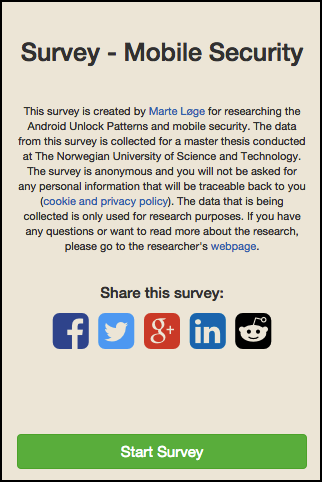
\includegraphics[scale=0.34]{pics/survey/start}
      }
      \subfigure[ALP introduction]{
        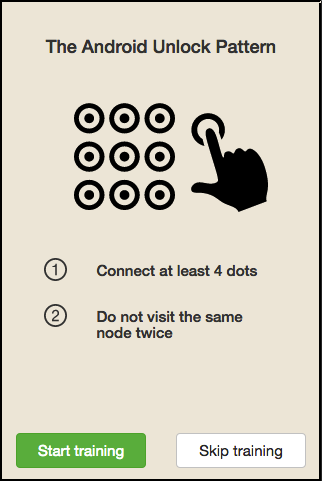
\includegraphics[scale=0.34]{pics/survey/rules}
      }
      \subfigure[Training mode]{
        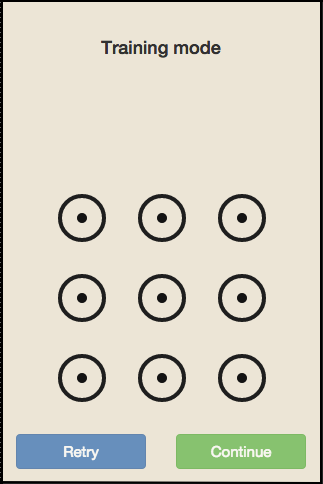
\includegraphics[scale=0.34]{pics/survey/training}
      }
      \caption{Survey screens}
    \end{figure}

    \begin{figure}[H]
      \centering
      \subfigure[Introduction to patterns]{
        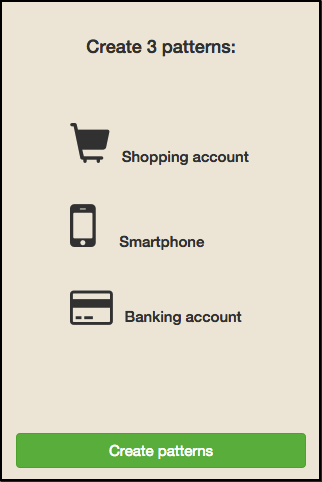
\includegraphics[scale=0.3]{pics/survey/pattern-introduction}
      }
      \subfigure[Shopping pattern]{
        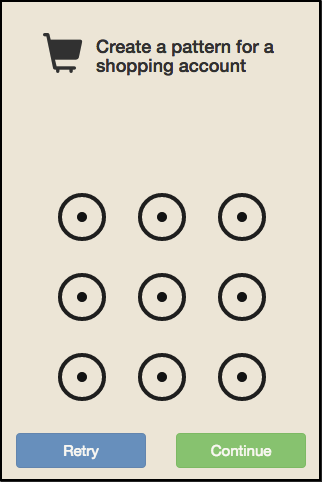
\includegraphics[scale=0.3]{pics/survey/shopping}
      }
      \subfigure[Smartphone pattern]{
        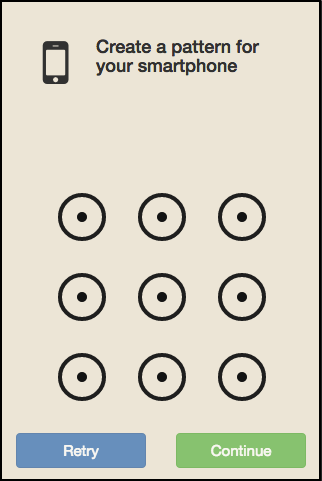
\includegraphics[scale=0.3]{pics/survey/smartphone}
      }
      \subfigure[Bank pattern]{
        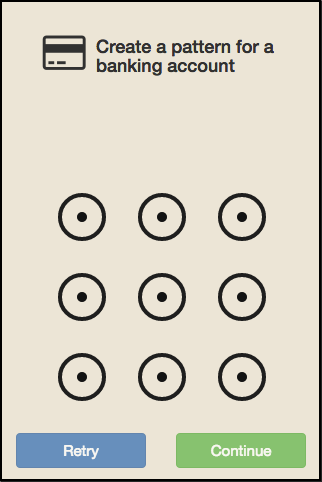
\includegraphics[scale=0.3]{pics/survey/bank}
      }
      \subfigure[Pattern length too short]{
        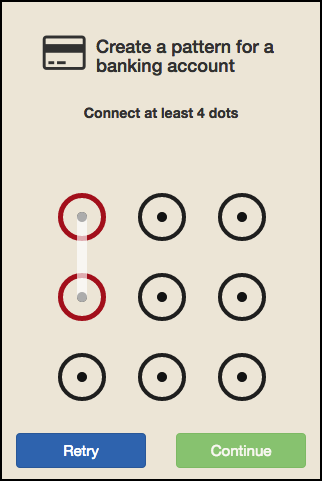
\includegraphics[scale=0.3]{pics/survey/not-valid-pattern-bank}
      }
      \subfigure[Valid pattern recorded]{
        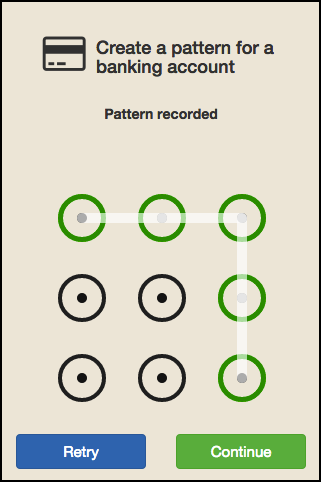
\includegraphics[scale=0.3]{pics/survey/pattern-recorded-bank}
      }
      \subfigure[Retype pattern]{
        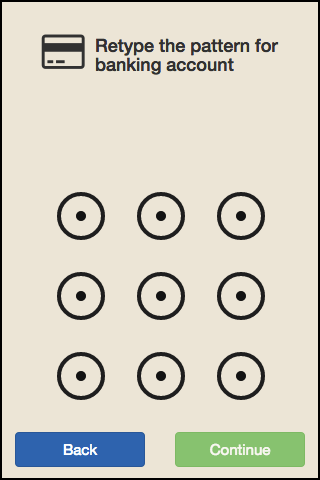
\includegraphics[scale=0.3]{pics/survey/retype-bank}
      }
      \subfigure[Not the same pattern]{
        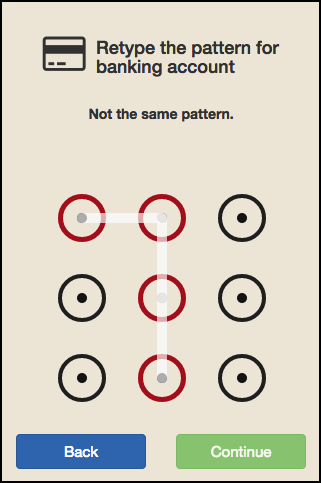
\includegraphics[scale=0.3]{pics/survey/not-valid-retype-bank}
      }
      \subfigure[Retype correct]{
        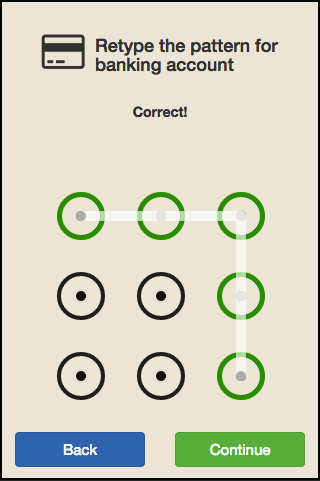
\includegraphics[scale=0.3]{pics/survey/retype-correct-bank}
      }
      \caption{Survey - Create and retye patterns}
    \end{figure}

    \begin{figure}[H]
      \centering
      \subfigure[Handsize]{
        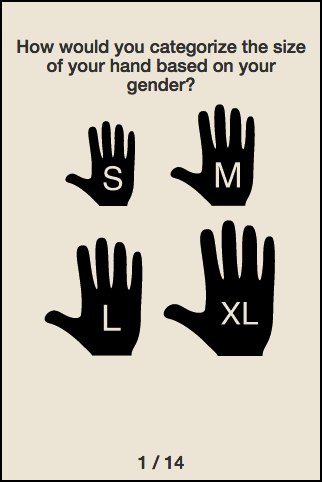
\includegraphics[scale=0.3]{pics/survey/handsize}
      }
      \subfigure[Handedness]{
        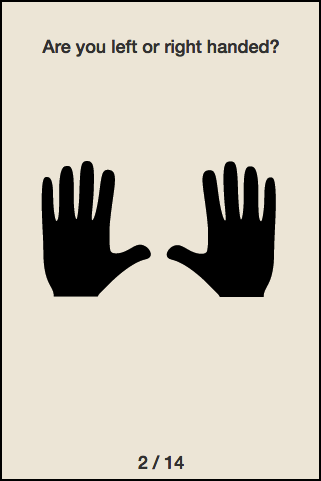
\includegraphics[scale=0.3]{pics/survey/handedness1}
      }
      \subfigure[Screen size]{
        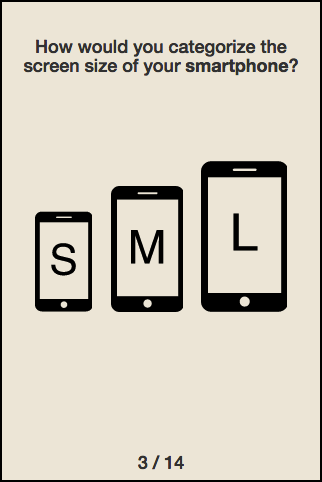
\includegraphics[scale=0.3]{pics/survey/screen}
      }
      \subfigure[Hand used when creating pattern]{
        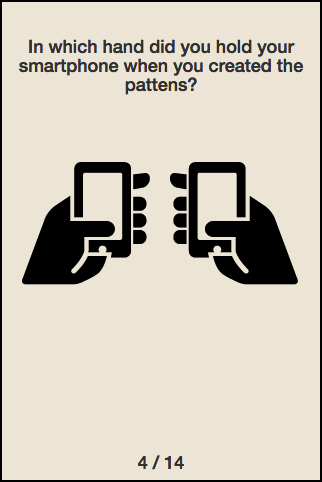
\includegraphics[scale=0.3]{pics/survey/handedness2}
      }
      \subfigure[Finger used]{
        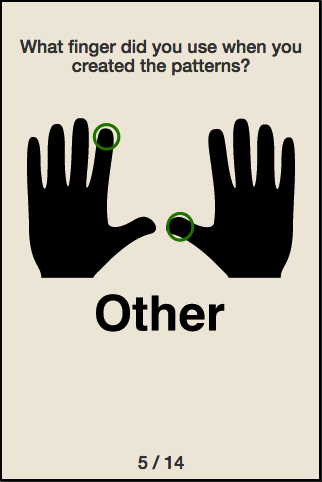
\includegraphics[scale=0.3]{pics/survey/finger}
      }
      \subfigure[Reading/writing direction]{
        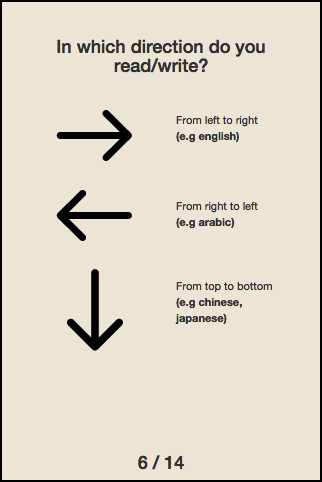
\includegraphics[scale=0.3]{pics/survey/reading}
      }
      \subfigure[Gender]{
        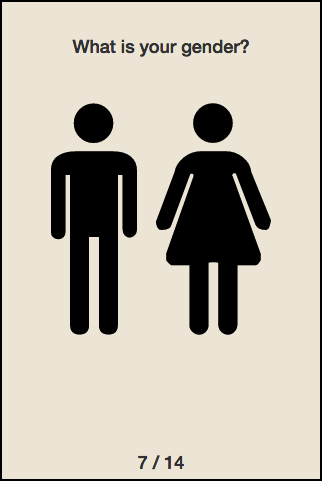
\includegraphics[scale=0.3]{pics/survey/gender}
      }
      \subfigure[Age]{
        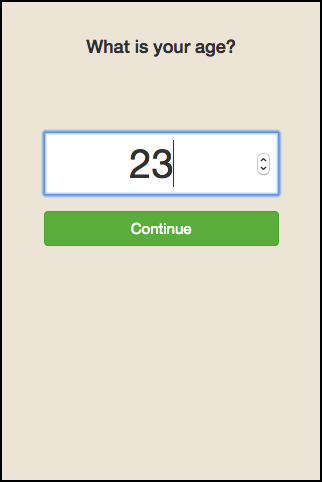
\includegraphics[scale=0.3]{pics/survey/age-2}
      }
      \caption{Survey - Questions}
    \end{figure}

    \begin{figure}[H]
      \centering
      \subfigure[Start screen]{
        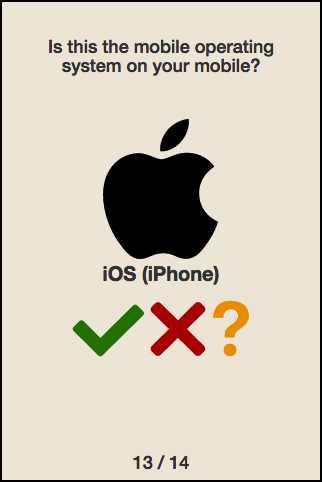
\includegraphics[scale=0.34]{pics/survey/ios}
      }
      \subfigure[ALP introduction]{
        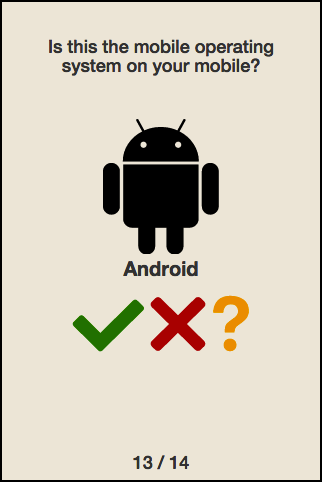
\includegraphics[scale=0.34]{pics/survey/android}
      }
      \subfigure[Training mode]{
        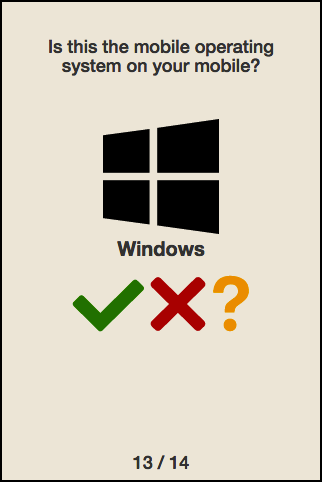
\includegraphics[scale=0.34]{pics/survey/windows}
      }
      \caption{Survey - Mobile OS}
    \end{figure}

    \begin{figure}[H]
      \centering
      \subfigure[Select icon]{
        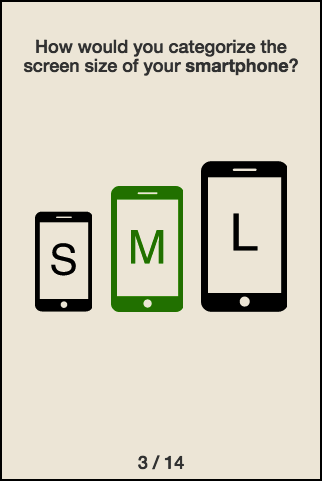
\includegraphics[scale=0.34]{pics/survey/icon-selected-1}
      }
      \subfigure[Icon fading out]{
        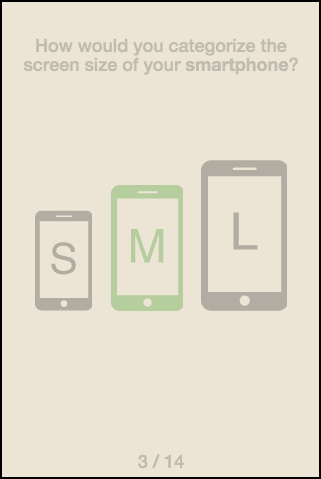
\includegraphics[scale=0.34]{pics/survey/icon-selected-3}
      }
      \subfigure[Icon faded out]{
        
\includegraphics[scale=0.34]{pics/survey/icon-selected-4}
      }
      \caption{Survey - Icon selecting effect}
    \end{figure}

\subsection{Technical Description of The Survey Application}

